\chapter{Host company introduction}

\startcontents[chapters]
\printmyminitoc{
	In this chapter, I would like to introduce the company that I am currently working on, Société française du radiotéléphone (SFR). It covers the sector of activity, the history of the company, its values and the most important part is how it is related to the master's that I am currently pursuing at Université Paris-Saclay.
}

\section{Sector of Activity}

Société française du radiotéléphone (SFR), is a French telecommunications company. It is the second oldest mobile network operator in France, after Orange and the second largest telecommunications company in France, also behind Orange.

SFR operates in the telecommunications sector, providing a wide range of communication and connectivity services to both individual consumers and businesses. The company's core activities include:

\begin{itemize}

    \item  Mobile services: offers mobile voice and data services, allowing customers to make calls, send messages, and access the internet on their smartphones and other mobile devices.

    \item Fixed-line services: provides fixed-line telephone services, including landline phone connections for homes and businesses.

    \item Internet services: offers broadband and high-speed internet connections, enabling customers to access the internet at home or work.

    \item Television services: deliver television services, including digital TV channels, on-demand content, and interactive features.

\end{itemize}

\begin{figure}[H]
    \centering
    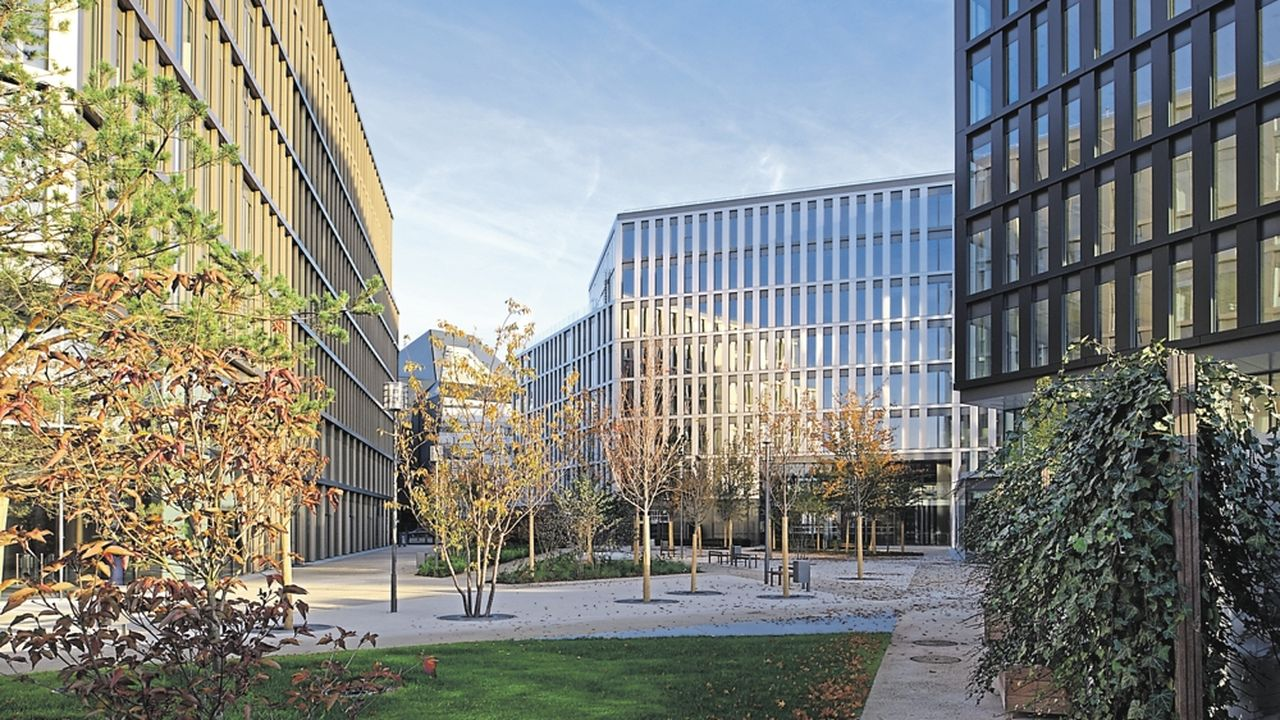
\includegraphics[width=0.9\textwidth]{images/altice-campus.jpg}
    \caption{A part of the current campus at 15ème arrondissement}
    \label{fig:altice_campus}
\end{figure}

SFR is known for its convergence strategy, which involves bundling multiple services, such as mobile, fixed-line, internet, and television, into comprehensive packages for customers seeking integrated communication and entertainment solutions.

Besides the representation of SFR in the Business-to-Consumer market, the company also serves the Business-to-Business market by offering tailored communication and connectivity solutions to support various industries and organizations.

\section{History}

\begin{figure}[H]
    \centering
    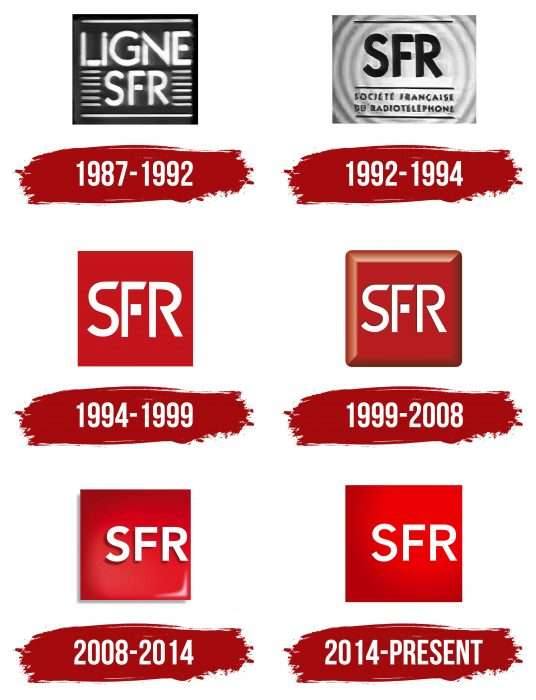
\includegraphics[width=0.4\textwidth]{images/SFR-Logo-History.jpg} % Replace "example-image.jpg" with the actual filename of your image
    \caption{History of SFR logo over time}
    \label{fig:sfr_logo}
\end{figure}

\begin{itemize}

    \item Founding Years and Early Growth (1987-2000):

SFR was established in 1987 as a subsidiary of Compagnie Générale des Eaux (now Veolia Environnement). The company's inception marked a significant step in introducing mobile telecommunications services to France.

    \item Expansion and Technological Advancements (2000s):

In the early 2000s, SFR launched its 3G (third generation) network, marking a milestone in mobile data services. The company's commitment to innovation and network improvement led to expanded coverage and enhanced service quality.

    \item Mergers and Acquisitions - Altice Era (2014):

In 2014, a major turning point occurred when Altice, a prominent cable and telecom company led by entrepreneur Patrick Drahi, acquired a controlling stake in SFR. This acquisition initiated a period of transformation and strategic repositioning for SFR within the Altice Group.

Under Altice's ownership, SFR underwent a series of changes aimed at convergence and diversification. The company focused on providing bundled services that combined mobile, fixed-line, internet, and television offerings, catering to customers' diverse communication and entertainment needs.

    \item Innovation and 5G Era (2020s):

Continuing its legacy of innovation, SFR, under the guidance of Altice, played a pivotal role in the deployment of 5G technology in France. This next-generation wireless technology promised higher speeds and improved connectivity, further solidifying SFR's position as a technological pioneer in the telecommunications landscape.

Throughout its history, SFR's journey has been closely intertwined with its affiliation with Altice, which brought new strategies, innovation, and growth opportunities. The partnership between SFR and Altice continues to shape the telecommunications landscape in France and beyond.

\end{itemize}

\section{Values}

SFR is built upon a foundation of core values that guide its operations and interactions:


\begin{itemize}

    \item \textbf{Innovation}
    
    SFR fosters a culture of continuous innovation, driving the development of cutting-edge solutions to meet the evolving needs of its customers.
    
    \item \textbf{Customer-Centric}
    
    The company is dedicated to delivering exceptional customer experiences, placing customer satisfaction at the heart of its strategies.
    
    \item \textbf{Collaboration}
    
    SFR values collaboration and teamwork, both within its internal teams and in partnership with external stakeholders.
    
    \item \textbf{Ethical Conduct}
    
    Ethical behavior and integrity are paramount in all aspects of SFR's operations, ensuring transparency and trust.
    
\end{itemize}

\section{Application of data in business operations}

Data can help businesses measure whether certain actions, products or services are profitable and where their greatest expenses might be. Identifying expenses is often the key to increasing profits because businesses can reduce those expenses and keep more of the revenue they earn.

SFR Analytics is one of the departments at SFR that takes care of data flow and data process. The department is divided into several groups, each group has its mission in the team.

\begin{itemize}
    \item Data science team
    \item Data analyst team
    \item Data governance team
\end{itemize}

I have been arranged to work in the data science team of SFR Analytics.

The main mission of the department is to manage and process the amount of data acquired by other departments to resolve the problem or to enhance the customer experience with the company. These are some of the missions that SFR Analytics is in charge of.

\begin{itemize}
    \item Reducing Churn Rate
    
SFR harnesses the power of AI and machine learning to analyze customer data and behavior patterns. By applying advanced predictive models, the company can identify potential churn indicators with greater accuracy. This enables SFR to proactively address customer concerns, tailor retention strategies, and offer personalized incentives, ultimately reducing churn rates. AI-driven insights empower SFR to anticipate customer needs, enhance service offerings, and strengthen customer relationships.

    \item Image Processing for Infrastructure Optimization
    
In its commitment to delivering optimal network performance, SFR employs AI-powered image processing techniques. By analyzing images and data collected from network infrastructure, AI algorithms can identify potential issues such as equipment damage or environmental factors that might affect network quality. This proactive approach allows SFR to swiftly address maintenance needs, minimize service disruptions, and ensure seamless connectivity for its customers.

    \item Natural Language Processing (NLP) in Call Centers
    
SFR revolutionizes its call center operations through the integration of natural language processing (NLP). AI-driven NLP models enable the automated analysis of customer interactions, extracting valuable insights from voice conversations, emails, and chat interactions. This not only enhances customer service quality by providing real-time assistance but also enables SFR to gain a deeper understanding of customer sentiments, preferences, and pain points. By leveraging NLP, SFR can fine-tune its services, optimize call center workflows, and continuously improve its offerings based on customer feedback.

    \item Predictive Analytics for Network Management
    
AI-driven predictive analytics play a vital role in optimizing SFR's network management. By analyzing vast amounts of network data, AI algorithms can forecast network congestion, identify potential areas of service degradation, and recommend proactive adjustments to ensure optimal network performance. This data-driven approach enhances user experiences, reduces downtime, and positions SFR as a provider of reliable and high-quality connectivity services.

\end{itemize}

SFR's strategic integration of artificial intelligence and machine learning into its business activities underscores the company's commitment to innovation and customer satisfaction. By leveraging AI-driven insights, SFR enhances its ability to reduce churn, optimize network infrastructure, elevate call center operations, and ensure seamless connectivity. These advancements not only propel SFR's growth but also contribute to its mission of delivering exceptional communication and digital services to its diverse customer base.